

\section{Data Retrieval} \label{Section: Testing Data Retrieval}

In Section \ref{Section: Data collection from the Router}, three different methods of data retrieval were implemented (Tampermonkey, Selenium WebDriver and SSH). All three methods principally worked the same, in that they periodically downloaded the database file every 5 seconds, but there are some core differences that set them apart. For instance Tampermonkey required the user to manually login to the ASUS Router and navigate to the data collection configuration page. From there the userscript would start the data collection process and download the database files. Due to the fact that Tampermonkey is a Google Chrome extension, the Chrome window must be kept open and the userscript is not compatible with other internet browsers (but there are similar extensions for other browsers). Additionally, running the data retrieval process on Google Chrome is resource intensive because of the inherent resource hog nature of its design. Using Selenium WebDriver, the login and navigation to the configuration page is automatically completed by the program. From there the Python script will start the data collection and download the database files. Selenium WebDriver uses ChromeDriver as the main interface for the data retrieval process, and once again this application must be kept open for the duration of the data collection process and due to its use of Chrome it is also resource intensive. The SSH method will connect and login to the ASUS router and periodically download the database file. All that is required of the user is to start the data collection process on the ASUS Web GUI, and from there the program will run in the background without the use of any other applications. 

With all three methods thoroughly tested and considered, the SSH method was chosen as the way to retrieve the from the ASUS router. The main reasons for this is the fact that this method is not dependent on any certain applications, it allows for the retrieval process to fully run in the background and is also the least resource intensive method.

\section{Data Collection For Testing}

In order to test the functionality of the Machine Learning model, data collection under specific environment conditions had to be conducted. Since data throughput is used as the main parameter for the ML classification, this parameter is also the main focus of the environment test. Initially datasets for training and testing were recorded while doing particular tasks such as downloading large files, watching high resolution videos and general web browsing in order to diversify the values of data throughput. However, this proved to be a very inefficient as it is difficult to control the actual values of data throughput recorded by the router. 

\subsection{StarTrinity Software: CST}

StarTrinity CST is a continuous internet speed test tool, which allows for long stress test duration with the download and upload bandwidth to be fixed \cite{CST}. This tool was used to generate test datasets with specific data throughput values, which fit within the ML classifications shown in Table \ref{table:class}. This tool is also used in the live testing and demonstration of the whole system in order to show the accuracy of the ML model across the entire range of data throughput values. 

\begin{figure} [ht]
    \centering
    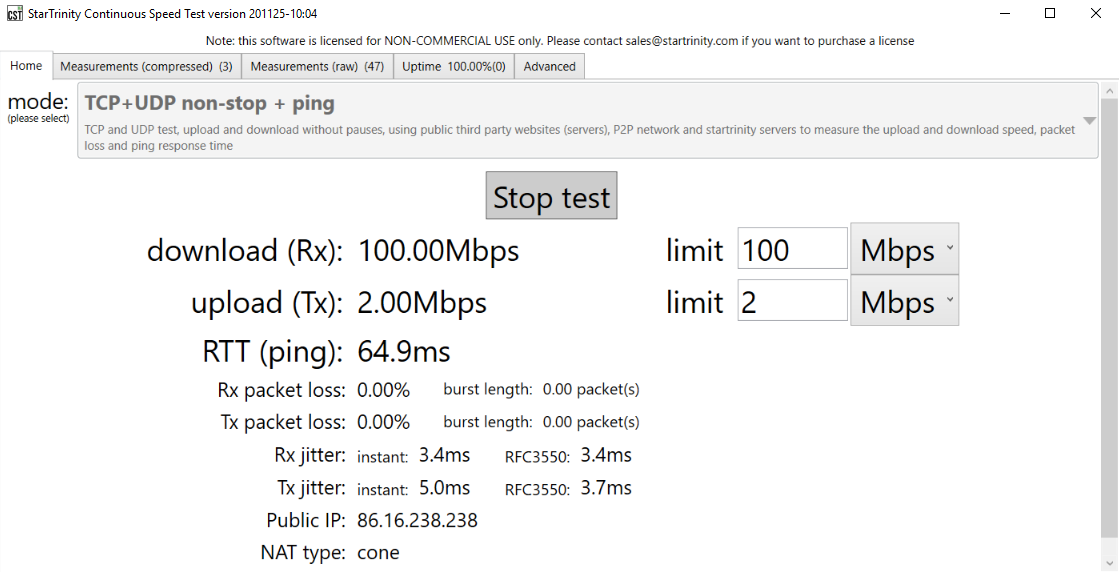
\includegraphics[width=1\linewidth]{pages/Chapter5/Chapter 5 images/CST.PNG}
    \caption{StarTrinity Software: Continuous Speed Test}
    \label{fig_CST}
\end{figure}

\section{Data Upload and Storage}

As mentioned in Chapter \ref{Chapter:System Design}, one of the telemetry pipelines is the direct upload of the data from the Laptop to the Cloud. This testing was conducted using the Selenium WebDriver to retrieve the data periodically, the script then detects a new database file and triggers the JSON conversion (Section \ref{section:Data Extraction}). Once this conversion is completed the files are uploaded to the Cloud (Section \ref{Section:pipeline1/3}). 

Figure \ref{fig_uploadData} shows the conversion functions operating, with their timings, and then the complete messages for the direct upload of data to the S3 Bucket with their respective timestamps. Figure \ref{fig_s3Upload} \& \ref{fig_s3UploadFolder} shows the data has been successfully uploaded along with .complete file. 

\begin{figure} [ht]
    \centering
    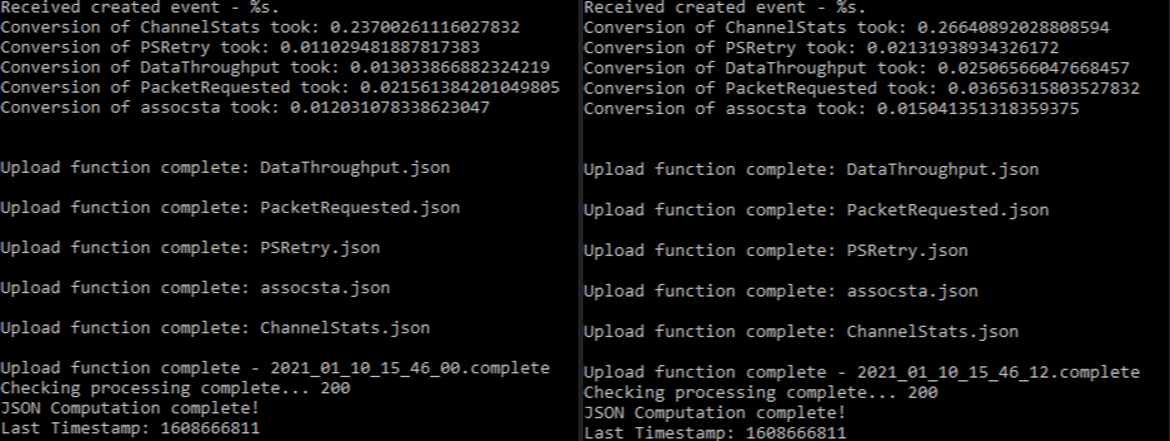
\includegraphics[width=1\linewidth]{pages/Chapter5/Chapter 5 images/dataUpload.PNG}
    \caption{Data Upload From Laptop Direct to S3 Bucket}
    \label{fig_uploadData}
\end{figure}

\begin{figure} [ht]
    \centering
    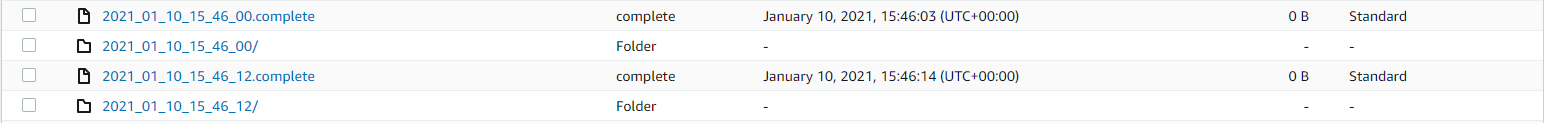
\includegraphics[width=1\linewidth]{pages/Chapter5/Chapter 5 images/s3Upload.PNG}
    \caption{S3 Bucket Proof of Upload with Data Folder and .complete File}
    \label{fig_s3Upload}
\end{figure}

\begin{figure} [ht]
    \centering
    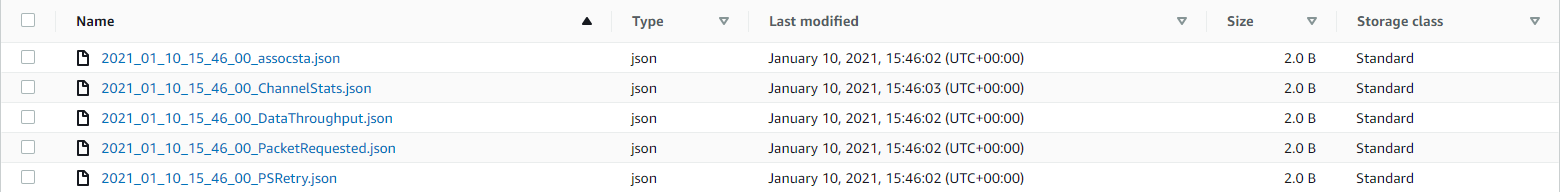
\includegraphics[width=1\linewidth]{pages/Chapter5/Chapter 5 images/s3UploadFolder.PNG}
    \caption{S3 Bucket Proof of Upload of Individual JSON Files}
    \label{fig_s3UploadFolder}
\end{figure}